% Options for packages loaded elsewhere
\PassOptionsToPackage{unicode}{hyperref}
\PassOptionsToPackage{hyphens}{url}
%
\documentclass[
]{book}
\usepackage{amsmath,amssymb}
\usepackage{lmodern}
\usepackage{iftex}
\ifPDFTeX
  \usepackage[T1]{fontenc}
  \usepackage[utf8]{inputenc}
  \usepackage{textcomp} % provide euro and other symbols
\else % if luatex or xetex
  \usepackage{unicode-math}
  \defaultfontfeatures{Scale=MatchLowercase}
  \defaultfontfeatures[\rmfamily]{Ligatures=TeX,Scale=1}
\fi
% Use upquote if available, for straight quotes in verbatim environments
\IfFileExists{upquote.sty}{\usepackage{upquote}}{}
\IfFileExists{microtype.sty}{% use microtype if available
  \usepackage[]{microtype}
  \UseMicrotypeSet[protrusion]{basicmath} % disable protrusion for tt fonts
}{}
\makeatletter
\@ifundefined{KOMAClassName}{% if non-KOMA class
  \IfFileExists{parskip.sty}{%
    \usepackage{parskip}
  }{% else
    \setlength{\parindent}{0pt}
    \setlength{\parskip}{6pt plus 2pt minus 1pt}}
}{% if KOMA class
  \KOMAoptions{parskip=half}}
\makeatother
\usepackage{xcolor}
\usepackage{color}
\usepackage{fancyvrb}
\newcommand{\VerbBar}{|}
\newcommand{\VERB}{\Verb[commandchars=\\\{\}]}
\DefineVerbatimEnvironment{Highlighting}{Verbatim}{commandchars=\\\{\}}
% Add ',fontsize=\small' for more characters per line
\usepackage{framed}
\definecolor{shadecolor}{RGB}{248,248,248}
\newenvironment{Shaded}{\begin{snugshade}}{\end{snugshade}}
\newcommand{\AlertTok}[1]{\textcolor[rgb]{0.94,0.16,0.16}{#1}}
\newcommand{\AnnotationTok}[1]{\textcolor[rgb]{0.56,0.35,0.01}{\textbf{\textit{#1}}}}
\newcommand{\AttributeTok}[1]{\textcolor[rgb]{0.77,0.63,0.00}{#1}}
\newcommand{\BaseNTok}[1]{\textcolor[rgb]{0.00,0.00,0.81}{#1}}
\newcommand{\BuiltInTok}[1]{#1}
\newcommand{\CharTok}[1]{\textcolor[rgb]{0.31,0.60,0.02}{#1}}
\newcommand{\CommentTok}[1]{\textcolor[rgb]{0.56,0.35,0.01}{\textit{#1}}}
\newcommand{\CommentVarTok}[1]{\textcolor[rgb]{0.56,0.35,0.01}{\textbf{\textit{#1}}}}
\newcommand{\ConstantTok}[1]{\textcolor[rgb]{0.00,0.00,0.00}{#1}}
\newcommand{\ControlFlowTok}[1]{\textcolor[rgb]{0.13,0.29,0.53}{\textbf{#1}}}
\newcommand{\DataTypeTok}[1]{\textcolor[rgb]{0.13,0.29,0.53}{#1}}
\newcommand{\DecValTok}[1]{\textcolor[rgb]{0.00,0.00,0.81}{#1}}
\newcommand{\DocumentationTok}[1]{\textcolor[rgb]{0.56,0.35,0.01}{\textbf{\textit{#1}}}}
\newcommand{\ErrorTok}[1]{\textcolor[rgb]{0.64,0.00,0.00}{\textbf{#1}}}
\newcommand{\ExtensionTok}[1]{#1}
\newcommand{\FloatTok}[1]{\textcolor[rgb]{0.00,0.00,0.81}{#1}}
\newcommand{\FunctionTok}[1]{\textcolor[rgb]{0.00,0.00,0.00}{#1}}
\newcommand{\ImportTok}[1]{#1}
\newcommand{\InformationTok}[1]{\textcolor[rgb]{0.56,0.35,0.01}{\textbf{\textit{#1}}}}
\newcommand{\KeywordTok}[1]{\textcolor[rgb]{0.13,0.29,0.53}{\textbf{#1}}}
\newcommand{\NormalTok}[1]{#1}
\newcommand{\OperatorTok}[1]{\textcolor[rgb]{0.81,0.36,0.00}{\textbf{#1}}}
\newcommand{\OtherTok}[1]{\textcolor[rgb]{0.56,0.35,0.01}{#1}}
\newcommand{\PreprocessorTok}[1]{\textcolor[rgb]{0.56,0.35,0.01}{\textit{#1}}}
\newcommand{\RegionMarkerTok}[1]{#1}
\newcommand{\SpecialCharTok}[1]{\textcolor[rgb]{0.00,0.00,0.00}{#1}}
\newcommand{\SpecialStringTok}[1]{\textcolor[rgb]{0.31,0.60,0.02}{#1}}
\newcommand{\StringTok}[1]{\textcolor[rgb]{0.31,0.60,0.02}{#1}}
\newcommand{\VariableTok}[1]{\textcolor[rgb]{0.00,0.00,0.00}{#1}}
\newcommand{\VerbatimStringTok}[1]{\textcolor[rgb]{0.31,0.60,0.02}{#1}}
\newcommand{\WarningTok}[1]{\textcolor[rgb]{0.56,0.35,0.01}{\textbf{\textit{#1}}}}
\usepackage{longtable,booktabs,array}
\usepackage{calc} % for calculating minipage widths
% Correct order of tables after \paragraph or \subparagraph
\usepackage{etoolbox}
\makeatletter
\patchcmd\longtable{\par}{\if@noskipsec\mbox{}\fi\par}{}{}
\makeatother
% Allow footnotes in longtable head/foot
\IfFileExists{footnotehyper.sty}{\usepackage{footnotehyper}}{\usepackage{footnote}}
\makesavenoteenv{longtable}
\usepackage{graphicx}
\makeatletter
\def\maxwidth{\ifdim\Gin@nat@width>\linewidth\linewidth\else\Gin@nat@width\fi}
\def\maxheight{\ifdim\Gin@nat@height>\textheight\textheight\else\Gin@nat@height\fi}
\makeatother
% Scale images if necessary, so that they will not overflow the page
% margins by default, and it is still possible to overwrite the defaults
% using explicit options in \includegraphics[width, height, ...]{}
\setkeys{Gin}{width=\maxwidth,height=\maxheight,keepaspectratio}
% Set default figure placement to htbp
\makeatletter
\def\fps@figure{htbp}
\makeatother
\setlength{\emergencystretch}{3em} % prevent overfull lines
\providecommand{\tightlist}{%
  \setlength{\itemsep}{0pt}\setlength{\parskip}{0pt}}
\setcounter{secnumdepth}{5}
\usepackage{booktabs}
\usepackage{amsthm}
\makeatletter
\def\thm@space@setup{%
  \thm@preskip=8pt plus 2pt minus 4pt
  \thm@postskip=\thm@preskip
}
\makeatother
\ifLuaTeX
  \usepackage{selnolig}  % disable illegal ligatures
\fi
\usepackage[]{natbib}
\bibliographystyle{apalike}
\IfFileExists{bookmark.sty}{\usepackage{bookmark}}{\usepackage{hyperref}}
\IfFileExists{xurl.sty}{\usepackage{xurl}}{} % add URL line breaks if available
\urlstyle{same} % disable monospaced font for URLs
\hypersetup{
  pdftitle={UCB Data Dictionary},
  pdfauthor={Ben Croft},
  hidelinks,
  pdfcreator={LaTeX via pandoc}}

\title{UCB Data Dictionary}
\author{Ben Croft}
\date{2022-09-07}

\begin{document}
\maketitle

{
\setcounter{tocdepth}{1}
\tableofcontents
}
\hypertarget{introduction}{%
\chapter{Introduction}\label{introduction}}

This book is a prototype of a functional \textbf{Data Dictionary}.

As a proof of concept, the book serves as a demonstration of what University of Colorado Boulder may adopt as \emph{open, collaborative, and living documentation} of data, data sets, and data applications. This proof of concept is version-controlled with Git, which enables version history, cross-team development, and rapid development. Additionally, this book can be hosted within Github Pages for public - or private - sharing among the campus system. Finally, this book can also be downloaded as a PDF, Ebook, or LaTeX file using the buttons at the top of this page.

\hypertarget{prerequisites}{%
\section{Prerequisites}\label{prerequisites}}

Since this data dictionary is written in Markdown, it can use anything that Pandoc's Markdown supports, e.g., a math equation \(a^2 + b^2 = c^2\).

The \textbf{bookdown} package can be installed from CRAN or Github:

\begin{Shaded}
\begin{Highlighting}[]
\FunctionTok{install.packages}\NormalTok{(}\StringTok{"bookdown"}\NormalTok{)}
\CommentTok{\# or the development version}
\CommentTok{\# devtools::install\_github("rstudio/bookdown")}
\end{Highlighting}
\end{Shaded}

Each Rmd file contains one and only one chapter, and a chapter is defined by the first-level heading \texttt{\#}.

To compile this example to PDF, you need XeLaTeX. You are recommended to install TinyTeX (which includes XeLaTeX): \url{https://yihui.name/tinytex/}.

\hypertarget{overview}{%
\chapter{Overview}\label{overview}}

The \textbf{Student Success Data Mart} provides the ability to review and manage analytics such as enrollment and registration metrics, count of student and faculty by registered courses, available courses for catalog building and schedule building, graduation rates and student career fulfillment of requirements, student academic standing, and faculty and student profiles.

Enrollment reports may include areas such as monitoring average class sizes, prerequisites not being met, grade distributions, and graduation eligibility.

Reports in this category can also include aggregated statistical reports with year-to-year comparisons in several subject areas.

\emph{With the Student Success Data Mart you can answer questions such as:}

\begin{verbatim}
1) What are the enrollment metrics for this term?
2) Can I get the Student Retention and Graduation rates year over year by Cohort, Gender and Ethnicity?
3) What is average GPA by Institution, Career and Program?
4) What is average time to graduate by Institution, Career and Program?
5) What classes are scheduled for this term?
6) Can I track and analyze the workload of the faculty?
7) What are the Class enrollment details?
8) What are the honors/awards details for the enrolled students?
\end{verbatim}

\hypertarget{where-does-the-student-success-data-mart-source-its-data-from}{%
\section{Where does the Student Success Data Mart source its data from?}\label{where-does-the-student-success-data-mart-source-its-data-from}}

Student Records Data Mart is related to the Academic Program Activation and Management business process. This business process includes Course Catalog, Class Scheduling, Student Career Term records and Enrollment business processes. These processes fulfill the institutions need to track course delivery, student participation through enrollments to those classes. The Academic Program activation and Management processes help manage class size, a student's enrollment in a class and track the resulting grades from the class.

\hypertarget{academic-plan-summary-star}{%
\chapter{Academic Plan Summary Star}\label{academic-plan-summary-star}}

\hypertarget{description}{%
\section{Description}\label{description}}

This star contains student summary entry for a given academic plan and related academic program.

Each row of this table contains the most current information about an individual student and a particular academic plan. This fact table also contains all students that enrolled, matriculated, withdrew, or completed the academic career/program and plan in the institution.

The table is \emph{not} keyed by term. \texttt{Institution}, \texttt{Career}, and \texttt{Program} are indirectly part of the key since they are derived from the \texttt{Academic\ Plan} dimension.

There is one row of data per student (person) academic plan surrogate ID and student career number.

Records are updated frequently, whenever the student program status changed. This may include status changes from activated, admitted, discontinued, or completed.

\hypertarget{helps-answer}{%
\section{Helps Answer}\label{helps-answer}}

This star may help answer the following:

\begin{itemize}
\tightlist
\item
  Number of enrollments by program or plan.
\item
  Number of students who dropped out.
\item
  Number of students in different program actions (statuses) and program action reasons by career, program, or plan.
\item
  Number of students that completed the program/plan.
\item
  Number of students that cancelled the program/plan.
\end{itemize}

\hypertarget{star-links}{%
\section{Star Links}\label{star-links}}

This star can be built from \texttt{F\_ACADPLAN\_SUMM} and connects to the following tables:

\begin{longtable}[t]{l}
\caption{\label{tab:table-data}A table generated by the longtable package.}\\
\toprule
matrix.input..ncol...1..byrow...T.\\
\midrule
PS\_D\_ACAD\_CAR\\
PS\_D\_ACAD\_LOAD\\
PS\_D\_ACAD\_ORG\\
PS\_D\_ACAD\_PLAN\\
PS\_D\_ACAD\_PROG\\
\addlinespace
PS\_D\_ACAD\_SPLAN\\
PS\_D\_ADMIT\_TYPE\\
PS\_D\_AWD\\
PS\_D\_CAMPUS\\
PS\_D\_DAY\\
\addlinespace
PS\_D\_DEG\\
PS\_D\_DEG\_STAT\\
PS\_D\_INSTITUTION\\
PS\_D\_LOCATION\\
PS\_D\_PERSON\\
\addlinespace
PS\_D\_PERSON\_ADDR\\
PS\_D\_PERSON\_ATTR\\
PS\_D\_PERSON\_EMAIL\\
PS\_D\_PERSON\_PHONE\\
PS\_D\_PROG\_ACN\\
\addlinespace
PS\_D\_PROG\_ACN\_RSN\\
PS\_D\_PROG\_STAT\\
PS\_D\_STDNT\_COHORT\\
PS\_D\_STDNT\_GRP\\
PS\_D\_TERM\\
\addlinespace
PS\_F\_ACADPLAN\_SUMM\\
PS\_R\_ACAD\_SPLAN\\
PS\_R\_AWD\\
PS\_R\_STDNT\_GRP\\
\bottomrule
\end{longtable}

\hypertarget{term-enrollment-star}{%
\chapter{Term Enrollment Star}\label{term-enrollment-star}}

\hypertarget{description-1}{%
\section{Description}\label{description-1}}

This star contains information regarding term enrollments by student. The star provides term statistics and cumulative statistics by term, student, institution, and career. This star also provides measures such as units-in-progress, GPA, number of courses enrolled, etc.

Institution and Career are indirectly part of the key since they are deirved from the Term surrogate ID.

There is one row of data per term surrogate ID and student.

\hypertarget{helps-answer-1}{%
\section{Helps Answer}\label{helps-answer-1}}

This star may help answer the following:

\begin{itemize}
\tightlist
\item
  Top student academic standings.
\item
  Nmber of units in progress vs.~passed by institution, career, program, or plan.
\item
  Average number of courses a student takes per term, by career, program, or plan.
\item
  Number of units a student is enrolled in.
\item
  Number of full time and part time students by term, institution, campus, primary program, etc.
\item
  Number of students taking GPA units.
\item
  Enrollment analysis by primary program and plan, term, institution, campus career, and program.
\end{itemize}

\hypertarget{star-links-1}{%
\section{Star Links}\label{star-links-1}}

This star can be built from \texttt{F\_TERM\_ENRLMT} and connects to the following tables:

\begin{longtable}[t]{l}
\caption{\label{tab:table-data-term-enrollment}A table generated by the longtable package.}\\
\toprule
matrix.input..ncol...1..byrow...T.\\
\midrule
PS\_D\_ACAD\_LOAD\\
PS\_D\_ACAD\_LVL\\
PS\_D\_ACAD\_ORG\\
PS\_D\_ACAD\_PLAN\\
PS\_D\_ACAD\_PROG\\
\addlinespace
PS\_D\_ACAD\_STNDNG\\
PS\_D\_DAY\\
PS\_D\_PERSON\\
PS\_D\_PERSON\_ADDR\\
PS\_D\_PERSON\_ATTR\\
\addlinespace
PS\_D\_PERSON\_EMAIL\\
PS\_D\_PERSON\_PHONE\\
PS\_D\_PROG\_ACN\\
PS\_D\_PROG\_ACN\_RSN\\
PS\_D\_PROG\_STAT\\
\addlinespace
PS\_D\_RSDNCY\\
PS\_D\_STDNT\_COHORT\\
PS\_D\_STDNT\_GRP\\
PS\_D\_TERM\\
PS\_D\_YEAR\\
\addlinespace
PS\_R\_PERSON\_RSDNCY\\
PS\_R\_STDNT\_GRP\\
\bottomrule
\end{longtable}

\hypertarget{applications}{%
\chapter{Applications}\label{applications}}

Some \emph{significant} applications are demonstrated in this chapter.

\hypertarget{example-one}{%
\section{Example one}\label{example-one}}

\hypertarget{example-two}{%
\section{Example two}\label{example-two}}

\hypertarget{final-words}{%
\chapter{Final Words}\label{final-words}}

We have finished a nice book.

\hypertarget{intro}{%
\chapter{Introduction}\label{intro}}

You can label chapter and section titles using \texttt{\{\#label\}} after them, e.g., we can reference Chapter \ref{intro}. If you do not manually label them, there will be automatic labels anyway, e.g., Chapter \ref{methods}.

Figures and tables with captions will be placed in \texttt{figure} and \texttt{table} environments, respectively.

\begin{Shaded}
\begin{Highlighting}[]
\FunctionTok{par}\NormalTok{(}\AttributeTok{mar =} \FunctionTok{c}\NormalTok{(}\DecValTok{4}\NormalTok{, }\DecValTok{4}\NormalTok{, .}\DecValTok{1}\NormalTok{, .}\DecValTok{1}\NormalTok{))}
\FunctionTok{plot}\NormalTok{(pressure, }\AttributeTok{type =} \StringTok{\textquotesingle{}b\textquotesingle{}}\NormalTok{, }\AttributeTok{pch =} \DecValTok{19}\NormalTok{)}
\end{Highlighting}
\end{Shaded}

\begin{figure}

{\centering 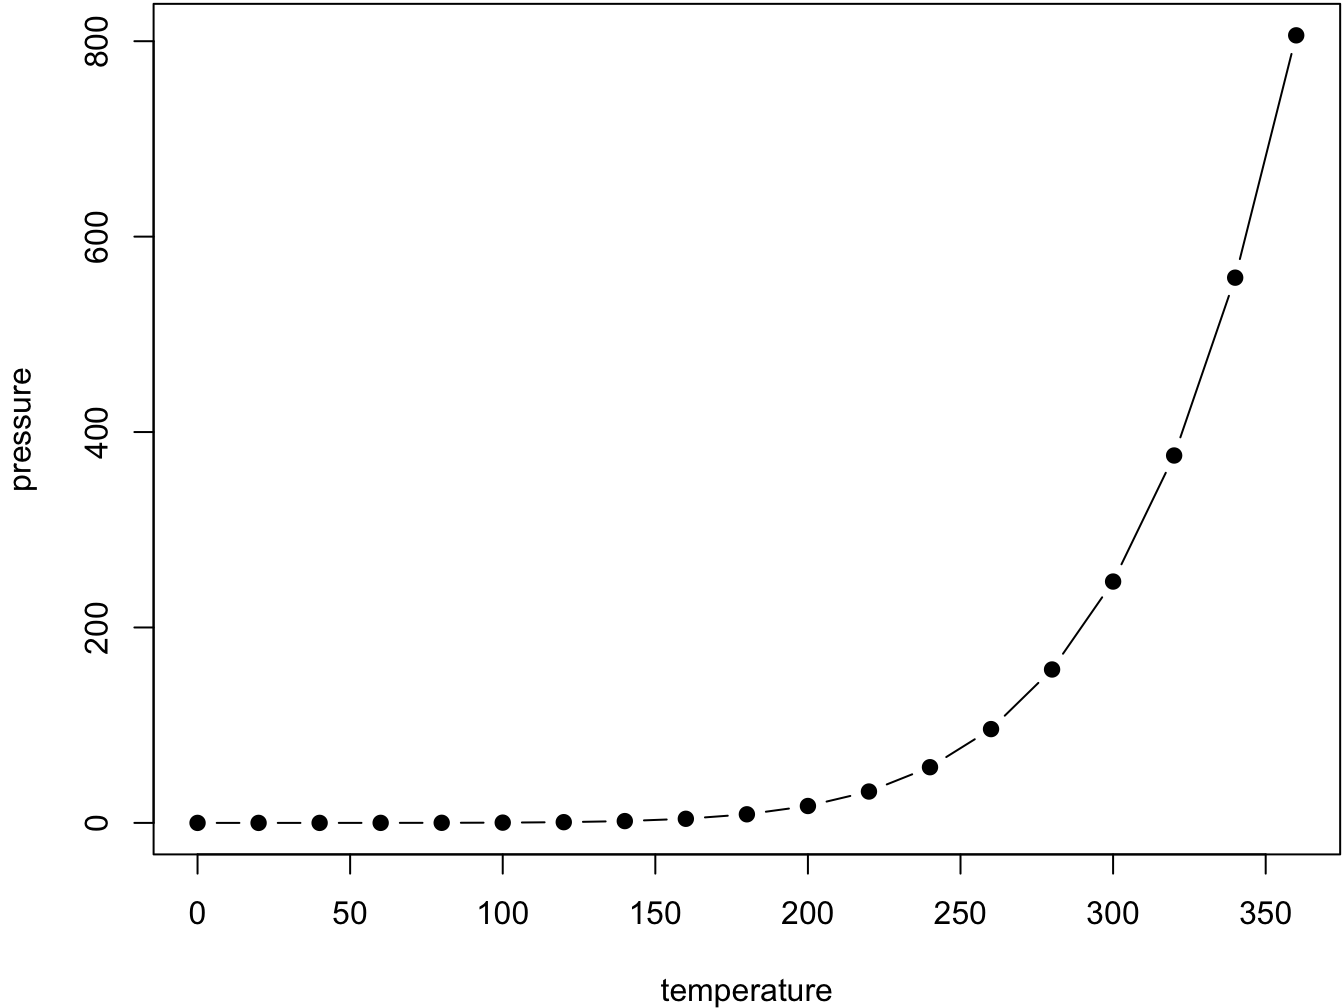
\includegraphics[width=0.8\linewidth]{UCB-Data-Dictionary_files/figure-latex/nice-fig-1} 

}

\caption{Here is a nice figure!}\label{fig:nice-fig}
\end{figure}

Reference a figure by its code chunk label with the \texttt{fig:} prefix, e.g., see Figure \ref{fig:nice-fig}. Similarly, you can reference tables generated from \texttt{knitr::kable()}, e.g., see Table \ref{tab:nice-tab}.

\begin{Shaded}
\begin{Highlighting}[]
\NormalTok{knitr}\SpecialCharTok{::}\FunctionTok{kable}\NormalTok{(}
  \FunctionTok{head}\NormalTok{(iris, }\DecValTok{20}\NormalTok{), }\AttributeTok{caption =} \StringTok{\textquotesingle{}Here is a nice table!\textquotesingle{}}\NormalTok{,}
  \AttributeTok{booktabs =} \ConstantTok{TRUE}
\NormalTok{)}
\end{Highlighting}
\end{Shaded}

\begin{table}

\caption{\label{tab:nice-tab}Here is a nice table!}
\centering
\begin{tabular}[t]{rrrrl}
\toprule
Sepal.Length & Sepal.Width & Petal.Length & Petal.Width & Species\\
\midrule
5.1 & 3.5 & 1.4 & 0.2 & setosa\\
4.9 & 3.0 & 1.4 & 0.2 & setosa\\
4.7 & 3.2 & 1.3 & 0.2 & setosa\\
4.6 & 3.1 & 1.5 & 0.2 & setosa\\
5.0 & 3.6 & 1.4 & 0.2 & setosa\\
\addlinespace
5.4 & 3.9 & 1.7 & 0.4 & setosa\\
4.6 & 3.4 & 1.4 & 0.3 & setosa\\
5.0 & 3.4 & 1.5 & 0.2 & setosa\\
4.4 & 2.9 & 1.4 & 0.2 & setosa\\
4.9 & 3.1 & 1.5 & 0.1 & setosa\\
\addlinespace
5.4 & 3.7 & 1.5 & 0.2 & setosa\\
4.8 & 3.4 & 1.6 & 0.2 & setosa\\
4.8 & 3.0 & 1.4 & 0.1 & setosa\\
4.3 & 3.0 & 1.1 & 0.1 & setosa\\
5.8 & 4.0 & 1.2 & 0.2 & setosa\\
\addlinespace
5.7 & 4.4 & 1.5 & 0.4 & setosa\\
5.4 & 3.9 & 1.3 & 0.4 & setosa\\
5.1 & 3.5 & 1.4 & 0.3 & setosa\\
5.7 & 3.8 & 1.7 & 0.3 & setosa\\
5.1 & 3.8 & 1.5 & 0.3 & setosa\\
\bottomrule
\end{tabular}
\end{table}

You can write citations, too. For example, we are using the \textbf{bookdown} package \citep{R-bookdown} in this sample book, which was built on top of R Markdown and \textbf{knitr} \citep{xie2015}.

\hypertarget{methods}{%
\chapter{Methods}\label{methods}}

We describe our methods in this chapter.

Math can be added in body using usual syntax like this

\hypertarget{math-example}{%
\section{math example}\label{math-example}}

\(p\) is unknown but expected to be around 1/3. Standard error will be approximated

\[
SE = \sqrt(\frac{p(1-p)}{n}) \approx \sqrt{\frac{1/3 (1 - 1/3)} {300}} = 0.027
\]

You can also use math in footnotes like this\footnote{where we mention \(p = \frac{a}{b}\)}.

We will approximate standard error to 0.027\footnote{\(p\) is unknown but expected to be around 1/3. Standard error will be approximated

  \[
  SE = \sqrt(\frac{p(1-p)}{n}) \approx \sqrt{\frac{1/3 (1 - 1/3)} {300}} = 0.027
  \]}

  \bibliography{book.bib,packages.bib}

\end{document}
